\section{Mathematical Morphology}

\paragraph*{}
Mathematical Morphology, born in 1960s and rapidly developing ever since, is both a theory and a technique for processing spatial structures. Soille described\cite{Soille03} the field as being \textit{mathematical} in that it is built upon set theory and geometry, and being \textit{morphology}\footnote{From Greek \textit{morphe} meaning form.} in that it aims at analyzing the shape of objects.

\paragraph*{}
In most general case, Mathematical Morphology applies to any complete lattice. We will concentrate on its application to region processing. In this context Mathematical Morphology can be looked at as a set of techniques that alter a region by probing it with another shape called kernel or structuring element.

\subsection{Kernel}

\paragraph*{}
Kernel in Mathematical Morphology is a shape that is repeatedly aligned at each position within the dimensions of the region being processed. At each such alignment the operator verifies how the aligned kernel fits in the region (e.g. if the kernel is contained in the region in its entirety) and depending on the results includes the location in the results or not.

\paragraph*{}
As kernel is pixel-precise binary shape itself, it can be represented as a region together with integer coordinates of its origin. Specifying the origin is important, as it is the position that will be aligned against the region being processed.

\gridDimensions{5}{5}

\newarray\kernelA
\readarray{kernelA}{%
0 & 0 & 0 & 0 & 0 &%
0 & 1 & 1 & 1 & 0 &%
0 & 1 & 2 & 1 & 0 &%
0 & 1 & 1 & 1 & 0 &%
0 & 0 & 0 & 0 & 0}

\newarray\kernelB
\readarray{kernelB}{%
0 & 0 & 0 & 0 & 0 &%
0 & 0 & 1 & 0 & 0 &%
0 & 1 & 2 & 1 & 0 &%
0 & 0 & 1 & 0 & 0 &%
0 & 0 & 0 & 0 & 0}

\newarray\kernelC
\readarray{kernelC}{%
0 & 0 & 0 & 0 & 0 &%
0 & 0 & 0 & 0 & 0 &%
0 & 0 & 2 & 1 & 0 &%
0 & 0 & 1 & 0 & 0 &%
0 & 0 & 0 & 0 & 0}


\begin{table}[h!]
\centering
\tabular{c c c}


\gridDimensions{5}{5}\begin{tikzpicture}[scale=0.40]\drawslabs{kernelA}\end{tikzpicture} &
\gridDimensions{5}{5}\begin{tikzpicture}[scale=0.40]\drawslabs{kernelB}\end{tikzpicture} &
\gridDimensions{5}{5}\begin{tikzpicture}[scale=0.40]\drawslabs{kernelC}\end{tikzpicture} 

\endtabular
\caption{Example kernels for morphological operations.}
\label{tab:MorphologyKernels}
\end{table}


\subsection{Dilation}

\paragraph*{}
First morphological operation that we are going to discuss is dilation. In this operator the kernel aligned at each position within the region dimensions needs to overlap with at least one pixel of the input region to include this position in the result:

\[
	Dilate(R,K) = \{[p_x,p_y] | R \cap Translate(K, [p_x,p_y]) \neq \emptyset \}
\] 

\newarray\dilationInput
\readarray{dilationInput}{%
0 & 0 & 0 & 0 & 0 & 0 & 0 &%
0 & 0 & 1 & 0 & 0 & 0 & 0 &%
0 & 1 & 0 & 1 & 1 & 1 & 0 &%
0 & 1 & 0 & 0 & 0 & 1 & 0 &%
0 & 0 & 0 & 0 & 0 & 0 & 0}

\newarray\dilationKernel
\readarray{dilationKernel}{%
0 & 0 & 0 & 0 & 0 &%
0 & 0 & 1 & 0 & 0 &%
0 & 1 & 2 & 1 & 0 &%
0 & 0 & 1 & 0 & 0 &%
0 & 0 & 0 & 0 & 0}

\newarray\dilationResult
\readarray{dilationResult}{%
0 & 0 & 1 & 0 & 0 & 0 & 0 &%
0 & 1 & 1 & 1 & 1 & 1 & 0 &%
1 & 1 & 1 & 1 & 1 & 1 & 1 &%
1 & 1 & 1 & 1 & 1 & 1 & 1 &%
0 & 1 & 0 & 0 & 0 & 1 & 0}

\begin{table}[h]
\centering
\tabular{c c c}

\gridDimensions{7}{5}\begin{tikzpicture}[scale=0.40]\drawslabs{dilationInput}\end{tikzpicture} &
\gridDimensions{5}{5}\begin{tikzpicture}[scale=0.40]\drawslabs{dilationKernel}\end{tikzpicture} &
\gridDimensions{7}{5}\begin{tikzpicture}[scale=0.40]\drawslabs{dilationResult}\end{tikzpicture} 

\\

$R$ &
$K$ &
$Dilate(R,K)$

\endtabular
\caption{Dilation of a region}
\label{tab:RegionDilation}
\end{table}

\paragraph*{}
If we decompose the kernel into its individual pixels we may observe that each such pixel $[k_x, k_y] \in K$ contributes a copy of the region translated by $[-k_x, -k_y]$ into the result. Therefore we may also define the dilation operator as follows:
\[
	Dilate(R,K) = \bigcup_{[k_x, k_y] \in K} Translate(R, [-k_x, -k_y])
\]

\paragraph*{}
Dilation effectively expands the region, the magnitude and direction of the expansion depending on the kernel being used. The operator is commonly used to join disconnected components of a region. Dilating a region by circular kernel of radius $r$ will expand the region uniformly in each direction up to distance of $r$ pixels, effectively joining region components separated by less than $2r$ pixels. One possible application is demonstrated in \reffig{DilationAppliedToFuses}.

\paragraph*{}
In this example we process a region representing metal parts of two fuses. As one of the fuses is burned out, the region contains three connected components. To split it into two connected components, each representing an individual fuse, we may perform the dilation before extracting the region components and intersect the resulting regions with the original one to preserve their original shape.

\begin{figure}
    \begin{subfigure}[b]{\basicWidth}
            \centering
            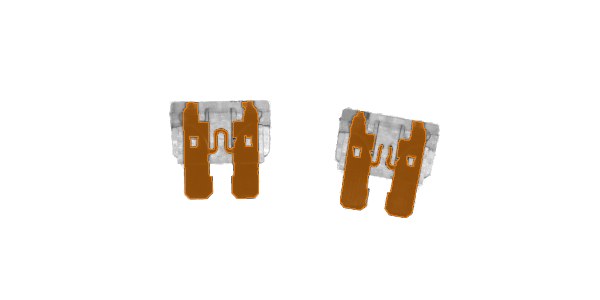
\includegraphics[width=\linewidth]{BlobAnalysis/img/fuses_region}
            \caption{}
    \end{subfigure}%
    ~
    \begin{subfigure}[b]{\basicWidth}
            \centering
            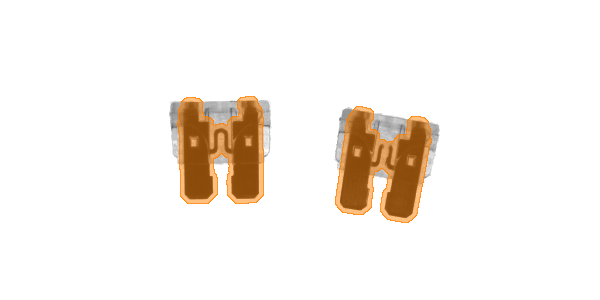
\includegraphics[width=\linewidth]{BlobAnalysis/img/fuses_dilated}
            \caption{}
    \end{subfigure}

    \begin{subfigure}[b]{\basicWidth}
            \centering
            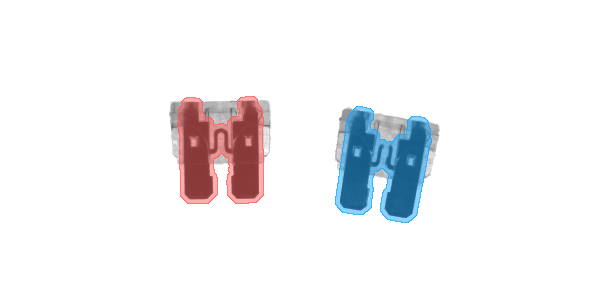
\includegraphics[width=\linewidth]{BlobAnalysis/img/fuses_dilated_blobs}
            \caption{}
    \end{subfigure}%
    ~
    \begin{subfigure}[b]{\basicWidth}
            \centering
            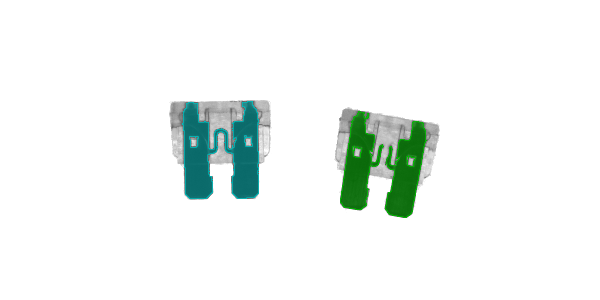
\includegraphics[width=\linewidth]{BlobAnalysis/img/fuses_components}
            \caption{}
    \end{subfigure}
    
    \caption{Dilation, extraction of connected components and intersection applied to split a region representing metal parts of the fuses (a) into components representing individual fuses (d).}
    \label{fig:DilationAppliedToFuses}
\end{figure}

\subsection{Erosion}

\paragraph*{}
Erosion is a shrinking counterpart of dilation. This operator requires that the aligned kernel is fully contained in the region being processed:

\[
	Erode(R,K) = \{[p_x,p_y] | Translate(K, [p_x,p_y]) \subseteq R \}
\] 

\newarray\erosionInput
\readarray{erosionInput}{%
0 & 0 & 1 & 0 & 0 & 0 & 0 &%
0 & 1 & 1 & 1 & 1 & 1 & 0 &%
1 & 1 & 1 & 1 & 1 & 1 & 1 &%
1 & 1 & 1 & 1 & 1 & 1 & 1 &%
0 & 1 & 0 & 0 & 0 & 1 & 0}

\newarray\erosionKernel
\readarray{erosionKernel}{%
0 & 0 & 0 & 0 & 0 &%
0 & 0 & 1 & 0 & 0 &%
0 & 1 & 2 & 1 & 0 &%
0 & 0 & 1 & 0 & 0 &%
0 & 0 & 0 & 0 & 0}

\newarray\erosionResult
\readarray{erosionResult}{%
0 & 0 & 0 & 0 & 0 & 0 & 0 &%
0 & 0 & 1 & 0 & 0 & 0 & 0 &%
0 & 1 & 1 & 1 & 1 & 1 & 0 &%
0 & 1 & 0 & 0 & 0 & 1 & 0 &%
0 & 0 & 0 & 0 & 0 & 0 & 0}

\begin{table}[h]
\centering
\tabular{c c c}

\gridDimensions{7}{5}\begin{tikzpicture}[scale=0.40]\drawslabs{erosionInput}\end{tikzpicture} &
\gridDimensions{5}{5}\begin{tikzpicture}[scale=0.40]\drawslabs{erosionKernel}\end{tikzpicture} &
\gridDimensions{7}{5}\begin{tikzpicture}[scale=0.40]\drawslabs{erosionResult}\end{tikzpicture} 

\\

$R$ &
$K$ &
$Erode(R,K)$

\endtabular
\caption{Erosion of a region}
\label{tab:RegionErosion}
\end{table}

\paragraph*{}
Similarly to dilation, we may also formulate erosion in terms of kernel decomposition. In this case each pixel of the kernel $[k_x, k_y] \in K$ also contributes the shifted copy of a region, but a position must be contained in all such contributions to be included in the results:
\[
	Erode(R,K) = \bigcap_{[k_x, k_y] \in K} Translate(R, [-k_x, -k_y])
\]

\paragraph*{}
The operations of dilation and erosion are closely related, but it is important to note that they are not inverse\footnote{Actually neither of these operation has an inverse, as such operation would have to magically guess where the lone pixels lost in erosion or holes filled in dilation were located.} of each other, i.e., erosion of a region does not necessarily \textit{cancel out} previously applied dilation; counterexample being presented in \reftab{RegionDilation} and \reftab{RegionErosion}. Quite contrary, consecutive application of dilation and erosion is extremely useful operation and will be discussed soon.

\paragraph*{}
Although dilation is not an inverse of erosion, another relation between the operations holds - they are duals of each other, meaning that dilation of a region is equivalent to erosion of its background (complement), and conversely.

\[
	Erode(R, K) = Dilate(R^{\complement}, K)^{\complement}
\]

\subsection{Closing}

\paragraph*{}
Before we define the next operator, let us get back for a moment to the dilation operator. As we remember, dilation expands the region in the way defined by the structuring element. It is worth noting that during this expansion small holes and region cavities may get completely filled in. This effect is worth attention as filling gaps of a region\footnote{Which could be introduced for instance by local glare of the lightning affecting the results of thresholding.} is a common need in industrial inspection.

\paragraph*{}
Unfortunately, dilation does not address this need precisely - the missing parts gets filled in, but also the region boundaries are expanded. It would be more convenient to have an operator that avoids the second effect while keeping the first.

\paragraph*{}
The closing operator addresses this need by dilating the region and eroding it right after that:
\[
	Close(R,K) = Erode(Dilate(R, K), Reflect(K))
\] 

\paragraph*{}
Initial dilation fills in the region gaps and the succeeding erosion brings the expanded region back to its original dimensions (but does not restore the gaps that were completely filled in). 

\paragraph*{}
It is worth noting that we use the reflected kernel for the second operation - if we recall that dilation may be formulated as a union of translations corresponding to individual pixels of the kernel ($\bigcup_{[k_x, k_y] \in K} Translate(R, [-k_x, -k_y])$), it is clear that we need to use the opposite translations to keep the region in its position.

\newarray\closingInput
\readarray{closingInput}{%
0 & 0 & 0 & 0 & 0 & 0 & 0 &%
0 & 0 & 1 & 0 & 0 & 0 & 0 &%
0 & 1 & 0 & 1 & 1 & 1 & 0 &%
0 & 1 & 0 & 0 & 0 & 1 & 0 &%
0 & 0 & 0 & 0 & 0 & 0 & 0}

\newarray\closingKernel
\readarray{closingKernel}{%
0 & 0 & 0 & 0 & 0 &%
0 & 0 & 1 & 0 & 0 &%
0 & 1 & 2 & 1 & 0 &%
0 & 0 & 1 & 0 & 0 &%
0 & 0 & 0 & 0 & 0}

\newarray\closingResult
\readarray{closingResult}{%
0 & 0 & 0 & 0 & 0 & 0 & 0 &%
0 & 0 & 1 & 0 & 0 & 0 & 0 &%
0 & 1 & 1 & 1 & 1 & 1 & 0 &%
0 & 1 & 0 & 0 & 0 & 1 & 0 &%
0 & 0 & 0 & 0 & 0 & 0 & 0}

\begin{table}[h]
\centering
\tabular{c c c}

\gridDimensions{7}{5}\begin{tikzpicture}[scale=0.40]\drawslabs{closingInput}\end{tikzpicture} &
\gridDimensions{5}{5}\begin{tikzpicture}[scale=0.40]\drawslabs{closingKernel}\end{tikzpicture} &
\gridDimensions{7}{5}\begin{tikzpicture}[scale=0.40]\drawslabs{closingResult}\end{tikzpicture} 

\\

$R$ &
$K$ &
$Close(R,K)$

\endtabular
\caption{Closing of a region}
\label{tab:RegionClosing}
\end{table}

\paragraph*{}
Closing is commonly applied whenever the extracted region contains gaps or cavities that should be filled in, an example of such application is demonstrated in \reffig{RegionClosingApplied}.

\twoFigures
{BlobAnalysis/img/morphology_close_before}
{BlobAnalysis/img/morphology_close_after}
{Closing operator used to fill gaps in a region.}
{RegionClosingApplied}
{\basicWidth}

\subsection{Opening}

\paragraph*{}
Another useful morphological operator is obtained by interchanging the order of operators that closing is composed of. The opening operator firstly erode a region and then dilates the result:

\[
	Open(R,K) = Dilate(Erode(R, K), Reflect(K))
\] 

\paragraph*{}
The effect of such composition is dual to the closing operator that we recently discussed. The initial erosion shrinks the region removing its isolated pixels and small branches, while the successive dilation brings it back to original dimensions, but cannot restore the parts that vanished completely during erosion.

\newarray\openingInput
\readarray{openingInput}{%
0 & 0 & 0 & 0 & 0 & 1 & 0 &%
0 & 0 & 1 & 0 & 0 & 0 & 0 &%
0 & 1 & 1 & 1 & 1 & 0 & 1 &%
1 & 1 & 1 & 0 & 0 & 0 & 0 &%
0 & 1 & 0 & 0 & 0 & 0 & 0}

\newarray\openingKernel
\readarray{openingKernel}{%
0 & 0 & 0 & 0 & 0 &%
0 & 0 & 1 & 0 & 0 &%
0 & 1 & 2 & 1 & 0 &%
0 & 0 & 1 & 0 & 0 &%
0 & 0 & 0 & 0 & 0}

\newarray\openingResult
\readarray{openingResult}{%
0 & 0 & 0 & 0 & 0 & 0 & 0 &%
0 & 0 & 1 & 0 & 0 & 0 & 0 &%
0 & 1 & 1 & 1 & 0 & 0 & 0 &%
1 & 1 & 1 & 0 & 0 & 0 & 0 &%
0 & 1 & 0 & 0 & 0 & 0 & 0}

\begin{table}[h]
\centering
\tabular{c c c}

\gridDimensions{7}{5}\begin{tikzpicture}[scale=0.40]\drawslabs{openingInput}\end{tikzpicture} &
\gridDimensions{5}{5}\begin{tikzpicture}[scale=0.40]\drawslabs{openingKernel}\end{tikzpicture} &
\gridDimensions{7}{5}\begin{tikzpicture}[scale=0.40]\drawslabs{openingResult}\end{tikzpicture} 

\\

$R$ &
$K$ &
$Open(R,K)$

\endtabular
\caption{Opening of a region}
\label{tab:RegionOpening}
\end{table}

\paragraph*{}
The opening operator may be applied to remove salt noise in the region or to eliminate its thin parts. Opening a region using a circular kernel of radius $r$ will remove all segments of the region that have less than $2r$ pixels in width (and keep the other parts intact). An example application is demonstrated in \reffig{RegionOpeningApplied}.

\twoFigures
{BlobAnalysis/img/morphology_open_before}
{BlobAnalysis/img/morphology_open_after}
{Opening operator used to determine excessively wide section of the rubber band.}
{RegionOpeningApplied}
{\basicWidth}

\begin{refImpl}
Basic morphological operators described in this section are available as \studio \,filters:
\begin{itemize}
    \item \filter{DilateRegion}{RegionMorphology}, \filter{DilateRegion\_AnyKernel}{RegionMorphology}
    \item \filter{ErodeRegion}{RegionMorphology}, \filter{ErodeRegion\_AnyKernel}{RegionMorphology}
    \item \filter{CloseRegion}{RegionMorphology}, \filter{CloseRegion\_AnyKernel}{RegionMorphology}
    \item \filter{OpenRegion}{RegionMorphology}, \filter{OpenRegion\_AnyKernel}{RegionMorphology}
\end{itemize}
The filters with \textit{\_AnyKernel} suffix allow to perform the operation using arbitrary kernel, while their counterparts allow to choose from a set of predefined, hard-coded kernels.
\end{refImpl}